\chapter{Runtimes}
\label{chap:runtimes}

Table \ref{tab:runtime-overview}

(Why different runtimes? Motivation?)

\begin{table}[htbp]
  \small
  \begin{tabular}{|c|c|c|c|c|c|}
    \hline
    \textbf{Runtime} & \textbf{Embeddable langs.}                                                                                               & \textbf{Architecture}                                                                                                & \textbf{Compiler}                                                         & \textbf{Compilation}                                        & \textbf{Platform}                                                                             \\ \hline
    Wasmtime         & Rust, Python                                                                                                                & \begin{tabular}[c]{@{}c@{}}x86, \\ x86\_64, \\ ARM\end{tabular}                                                      & \begin{tabular}[c]{@{}c@{}}Cranelift, \\ LLVM\end{tabular}                & JIT, AoT                                                    & \begin{tabular}[c]{@{}c@{}}Windows, \\ Linux, \\ Mac OS\end{tabular}                          \\ \hline
    Wasmer           & Rust, C++                                                                                                                   & \begin{tabular}[c]{@{}c@{}}x86, \\ x86\_64, \\ ARM\end{tabular}                                                      & \begin{tabular}[c]{@{}c@{}}Cranelift, \\ LLVM, \\ Singlepass\end{tabular} & JIT, AoT                                                    & \begin{tabular}[c]{@{}c@{}}Windows, \\ Linux, \\ Mac OS, \\ Free BSD, \\ Android\end{tabular} \\ \hline
    Wasm3            & \begin{tabular}[c]{@{}c@{}}Python3, Rust, \\ GoLang, \\ Zig, Perl, Swift, \\ C\# .NET\end{tabular}                          & \begin{tabular}[c]{@{}c@{}}x86, \\ x86\_64, \\ ARM, \\ RISC-V, \\ PowerPC, \\ MIPS, \\ Xtensa, \\ ARC32\end{tabular} & Custom                                                                    & Interpreter                                                 & \begin{tabular}[c]{@{}c@{}}Windows, \\ Linux, \\ Mac OS, \\ Free BSD, \\ Android\end{tabular} \\ \hline
    WasmEdge         & \begin{tabular}[c]{@{}c@{}}Solidity, Rust, \\ C++, TinyGo, \\ JavaScript, Python, \\ Grain, Swift,\\ Zig, Ruby\end{tabular} & \begin{tabular}[c]{@{}c@{}}x86, \\ x86\_64, \\ ARM\end{tabular}                                                      & LLVM                                                                      & \begin{tabular}[c]{@{}c@{}}Interpreter, \\ AoT\end{tabular} & \begin{tabular}[c]{@{}c@{}}Windows, \\ Linux, \\ Mac OS, \\ Android\end{tabular}              \\ \hline
  \end{tabular}
  \caption{WebAssembly Runtimes overview based on \cite{akinyemi_2023_awesome}}
  \label{tab:runtime-overview}
\end{table}
    

\section{Serverless Requirements}
\label{sec:serverless-requirements}

The following summary of requirements should be met by an ideal serverless runtime, therefore, we will use them as a guideline to evaluate the different runtimes.

A serverless runtime should be able to:

\begin{enumerate}
	\item Ensure security and isolation between functions.
	\item Have a small footprint to reduce the startup time of functions, therefore, a small memory footprint and also fast startup time. 
	\item Integrate effortlessly with existing frameworks. 
	\item Support multiple programming languages but not less to the traditional serverless platforms. 
	\item Execute functions with a speed comparable to native speed.
	\item Have the capability to run on various instruction set architectures, including but not limited to \texttt{x86\_64} and \texttt{arm}.
	\item Handle large amount of I/O operations concurrently.
\end{enumerate}

\section{Evaluation of features}
\label{sec:evaluation-of-features}

\section{Execution Models}
\label{sec:execution-models}

\subsection{JIT - Just In Time Compilation}
\label{sec:jit}

\subsection{Interpreter}
\label{sec:interpreter}

\subsection{WASM to native compilation}
\label{sec:wasm-to-native}

\subsection{AOT - Ahead Of Time Compilation}
\label{sec:aot}


\subsection{Wasm Snapshots (Wizer)}
\label{sec:wizer}

As noted earlier, for serverless functions, having a fast startup time is crucial. 
Thus, techniques that can remove the repetitive initialization step from the critical 
path are highly beneficial. Wizer is a tool that can create a snapshot of an already 
initialized WebAssembly module. The snapshot is a pre-initialized Wasm module that should start 
faster without sacrificing any security or portability. 

As shown in Figure \ref{fig:wizer}, a program needs to go through four phases before it can be executed. 
The steps can be divided into two sections - the time of the developer spends to build and upload the program and the time of the user waiting for the program to become interactive on each request. The user experience can be enhanced by reducing the time spent in the second section. 

\begin{figure}[H]
	\centering
	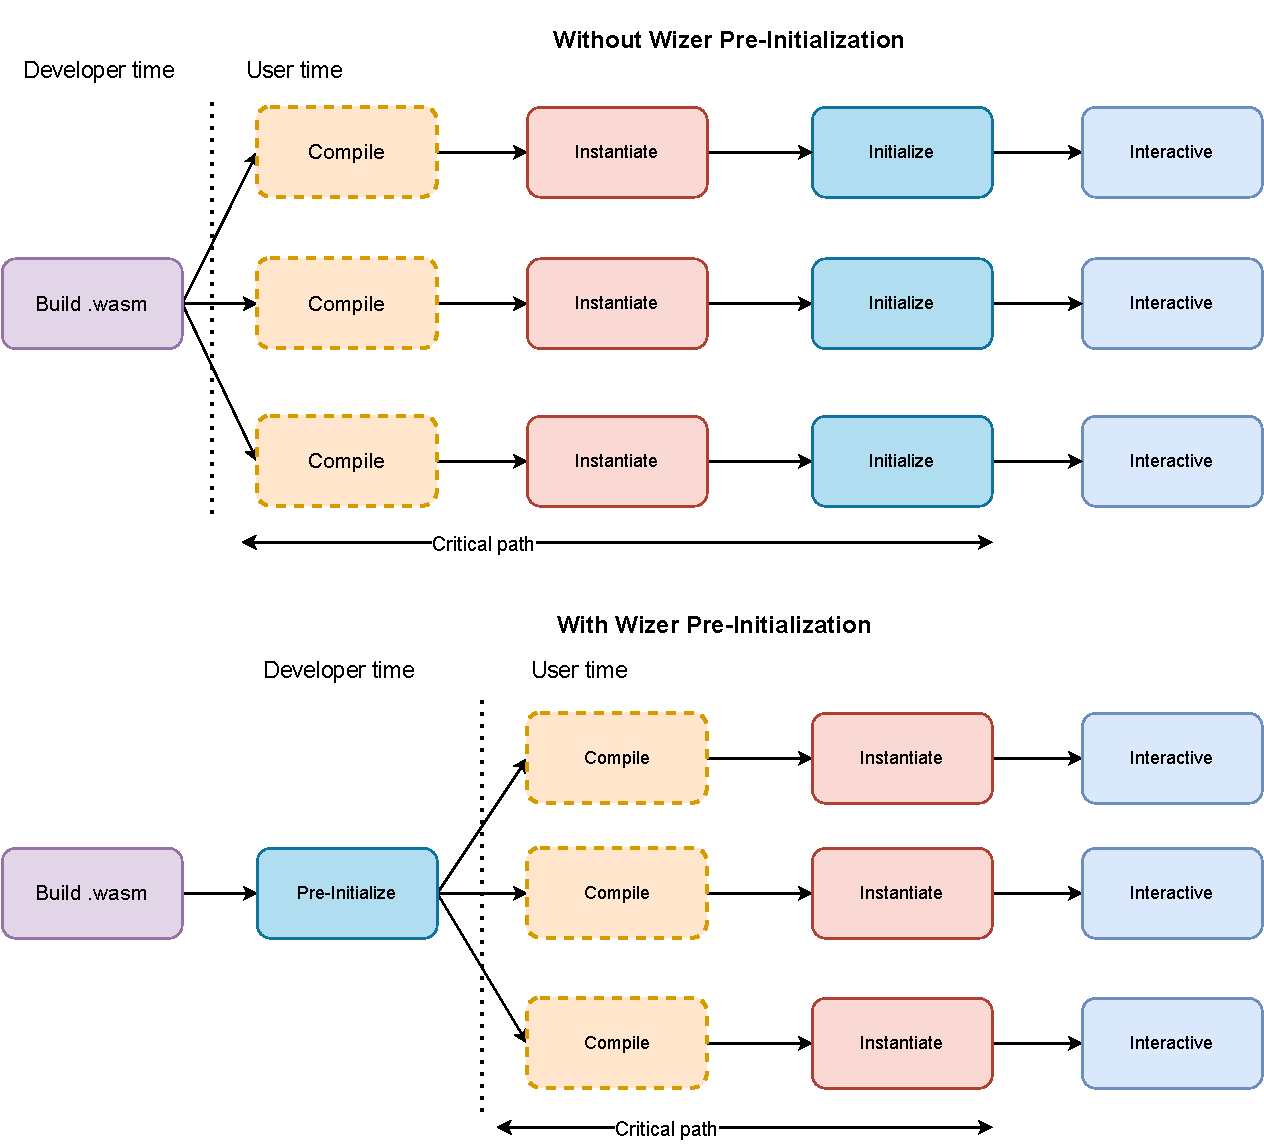
\includegraphics[width=0.8\linewidth]{images/runtimes/Wizer.drawio.pdf}
	\caption{Overview of Pre-initialization vs. Non Pre-initialization, based on \cite{fitzgerald_2021_hit}}
	\label{fig:wizer}
\end{figure}

Wizer creates a pre-initialized snapshot through these four phases \cite{fitzgerald_2021_hit}:
\begin{enumerate}
	\item Instrument: The first phase, known as the instrumentation phase, aims to export the internal state of the Wasm module so that Wizer can read it during the snapshot phase.
	\item Initialize: In the second phase, Wizer uses the Wasmtime runtime to compile and initialize the Wasm module. It then calls the exported "wizer.initialize" function.
	\item Snapshot: The third phase is the snapshot phase, in which Wizer reads the exports created in the first phase and generates the snapshot structure.
	\item Rewrite: The final phase is the rewrite phase. Wizer takes the initial Wasm module and the snapshot to create a new Wasm module. It removes the start section, as the snapshot has already executed the initializations, and updates each memory's minimum size to the size of the snapshot memories, as they may have grown during the initialization phase.
\end{enumerate}


\subsubsection{Wizer benchmarks}
\label{sec:wizer-benchmarks}

Initial benchmarks indicate that Wizer can provide between 1.35 and 6.00 times faster instantiation and initialization, depending on the specific workload. Running the benchmarks included in the Wizer repository \cite{bytecodealliance_2023_wizer}, we can confirm that Wizer can provide a significant speedup in the instantiation and initialization phases. For \ref{fig:uap-bench} we ran the User Agent Parsing benchmark from the Wizer repository. The benchmark creates a "RegexSet" using user agent parsing regexes from the Browserscope project. Then, it tests if the input string matches any known user agent patterns. 

Our results on the User Agent Benchmark shows 14 times faster instantiation more than double the speedup of the original benchmark. We used the newest version of Wizer and Wasmtime ran on a M1 Pro MacBook with 32GB of RAM.

However, there is a caveat to this benchmark, it is important to note that not all programs will experience enhancements in instantiation and startup latency. For instance, Wizer can frequently enlarge the Data section of a Wasm module, potentially leading to adverse effects on network transfer times for web applications. 

In the case of the User Agent Parsing benchmark, the orginal Wasm module is 3.1MB and the snapshot is 35.7MB. The size of the snapshot is 11.5 times larger than the original Wasm module. This is because the snapshot contains a large set of regexes in the data segment.
In the context of edge computing, this could be a problem, as the larger the Wasm module, the longer it takes to transfer it to the edge hosts. Furthermore, both Cloudflare and Fastly cache the executable code across their global network of edge servers. Thus, making this solution on some instances less desirable. 

\begin{figure}[H]
	\centering
	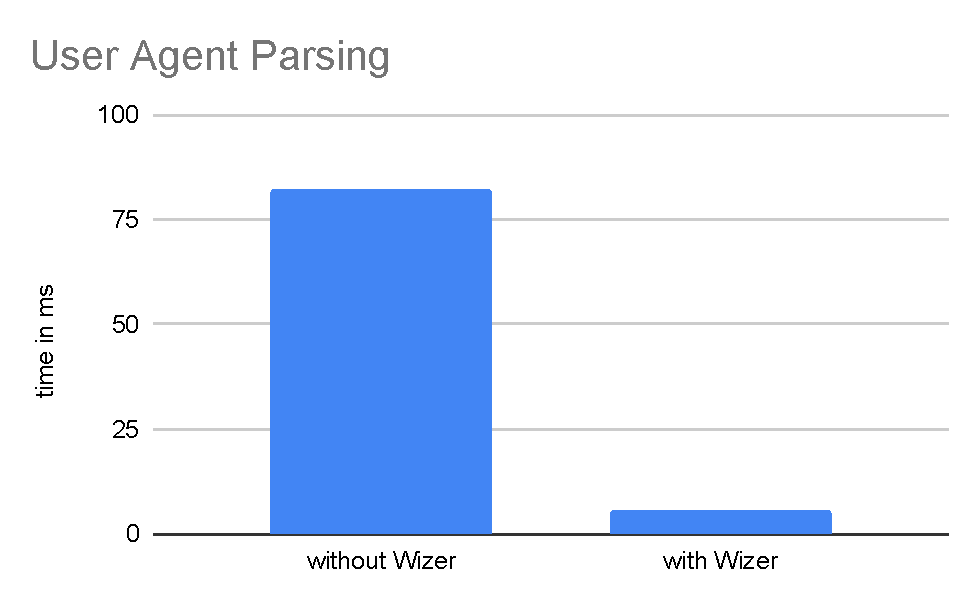
\includegraphics[width=0.6\linewidth]{images/runtimes/UAP.pdf}
	\caption{User Agent Parsing benchmark}
	\label{fig:uap-bench}
\end{figure}


\section{Comparison to V8 Isolates}
\label{sec:v8-comparison}
A V8 isolate is a separate instance of the V8 engine that has its own memory, garbage collector, and global object \cite{a2021_isolate}. An isolate can run scripts in a safe and isolated environment, without interfering with other isolates \cite{cloudflareinc_2023_how}. An isolate also has its own state, which means that objects from one isolate cannot be used in another isolate. When V8 is initialized, a default isolate is created and entered, but you can also create your own isolates using the V8 API \cite{a2021_isolate}.

\begin{figure}[H]
	\centering
		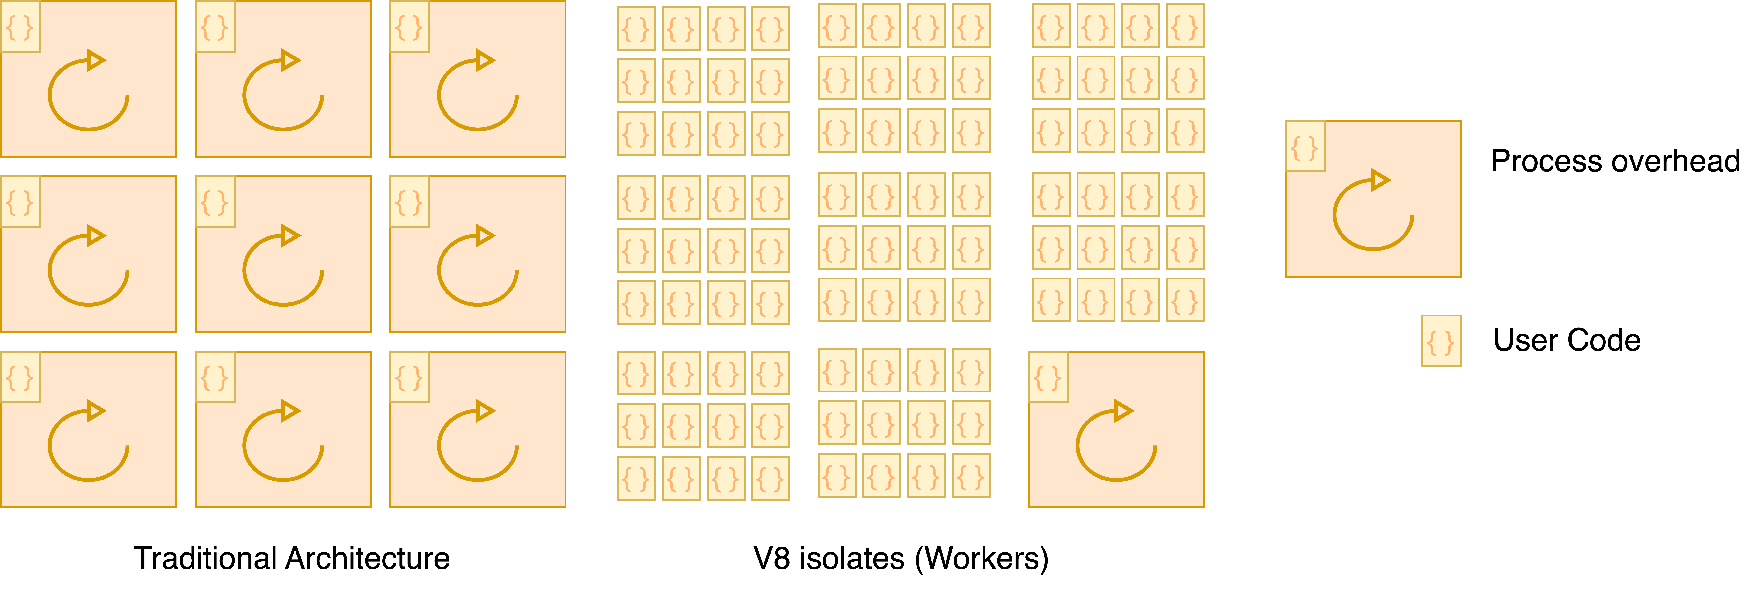
\includegraphics[width=\textwidth,height=\textheight,keepaspectratio]{images/runtimes/v8-isolates.pdf}
	\caption{containerized vs. \gls{V8} \glspl{isolate} figure redrawn from \cite{cloudflareinc_2023_how}}
	\label{fig:v8-isolates}
\end{figure}

\subsection{Advantages and disadvantages}
\label{sec:advantages-disadvantages}